\section{Simulation Analysis}
\label{sec:simulation}

In this section the circuit in figure \ref{fig:circuit} is simulated
using the software \textit{Ngspice}.

\subsection{Operating Point Analysis}

\subsubsection{t<0}

We started by simulating the static circuit for  $time (t) < 0$ and 
got the voltages and currents in each node and branch of the circuit.
Table \ref{tab:op_tabNodalSpice1} shows the simulated operating 
point results for the circuit under analysis.
Note that, because at $t<0$ the voltage is constant, the current through
the capacitor is zero, i.e., it can be replaced by an open circuit.

\hfill

\subsubsection{Equivalent Resistance}

Following this we replaced $V_s$ with a short circuit and substituted
the capacitor with a voltage source $Vx = V_8-V_6$, $V_8$ and $V_6$
being the potencial at nodes 8 and 6 previously calculated.
From this we obtained the values in table \ref{tab:op_tabReqSpice}. 

As explained in section , we had to substitute 
the capacitor with a voltage source because we cannot replace the 
independent source with short circuits or open circuits, as we did 
with $V_s$ and simply calculate the equivalent resistance using
simple resistance sum formula.

By comparing the results exposed in table \ref{tab:op_tabReqSpice} with the 
theoretical results in table \ref{tab:op_nodal5_tab}, we 
find that the results agree up to the last decimal place represented 
by \textit{Ngspice} (5 decimal places). This agreement can be explained 
with the fact that there are only linear and time independent components 
in the circuit we are considering.


\subsection{Transient Analysis}

In this section we analysed the response of the circuit for several
conditions.

\subsubsection{Natural Response}

\begin{figure}[h] \centering
  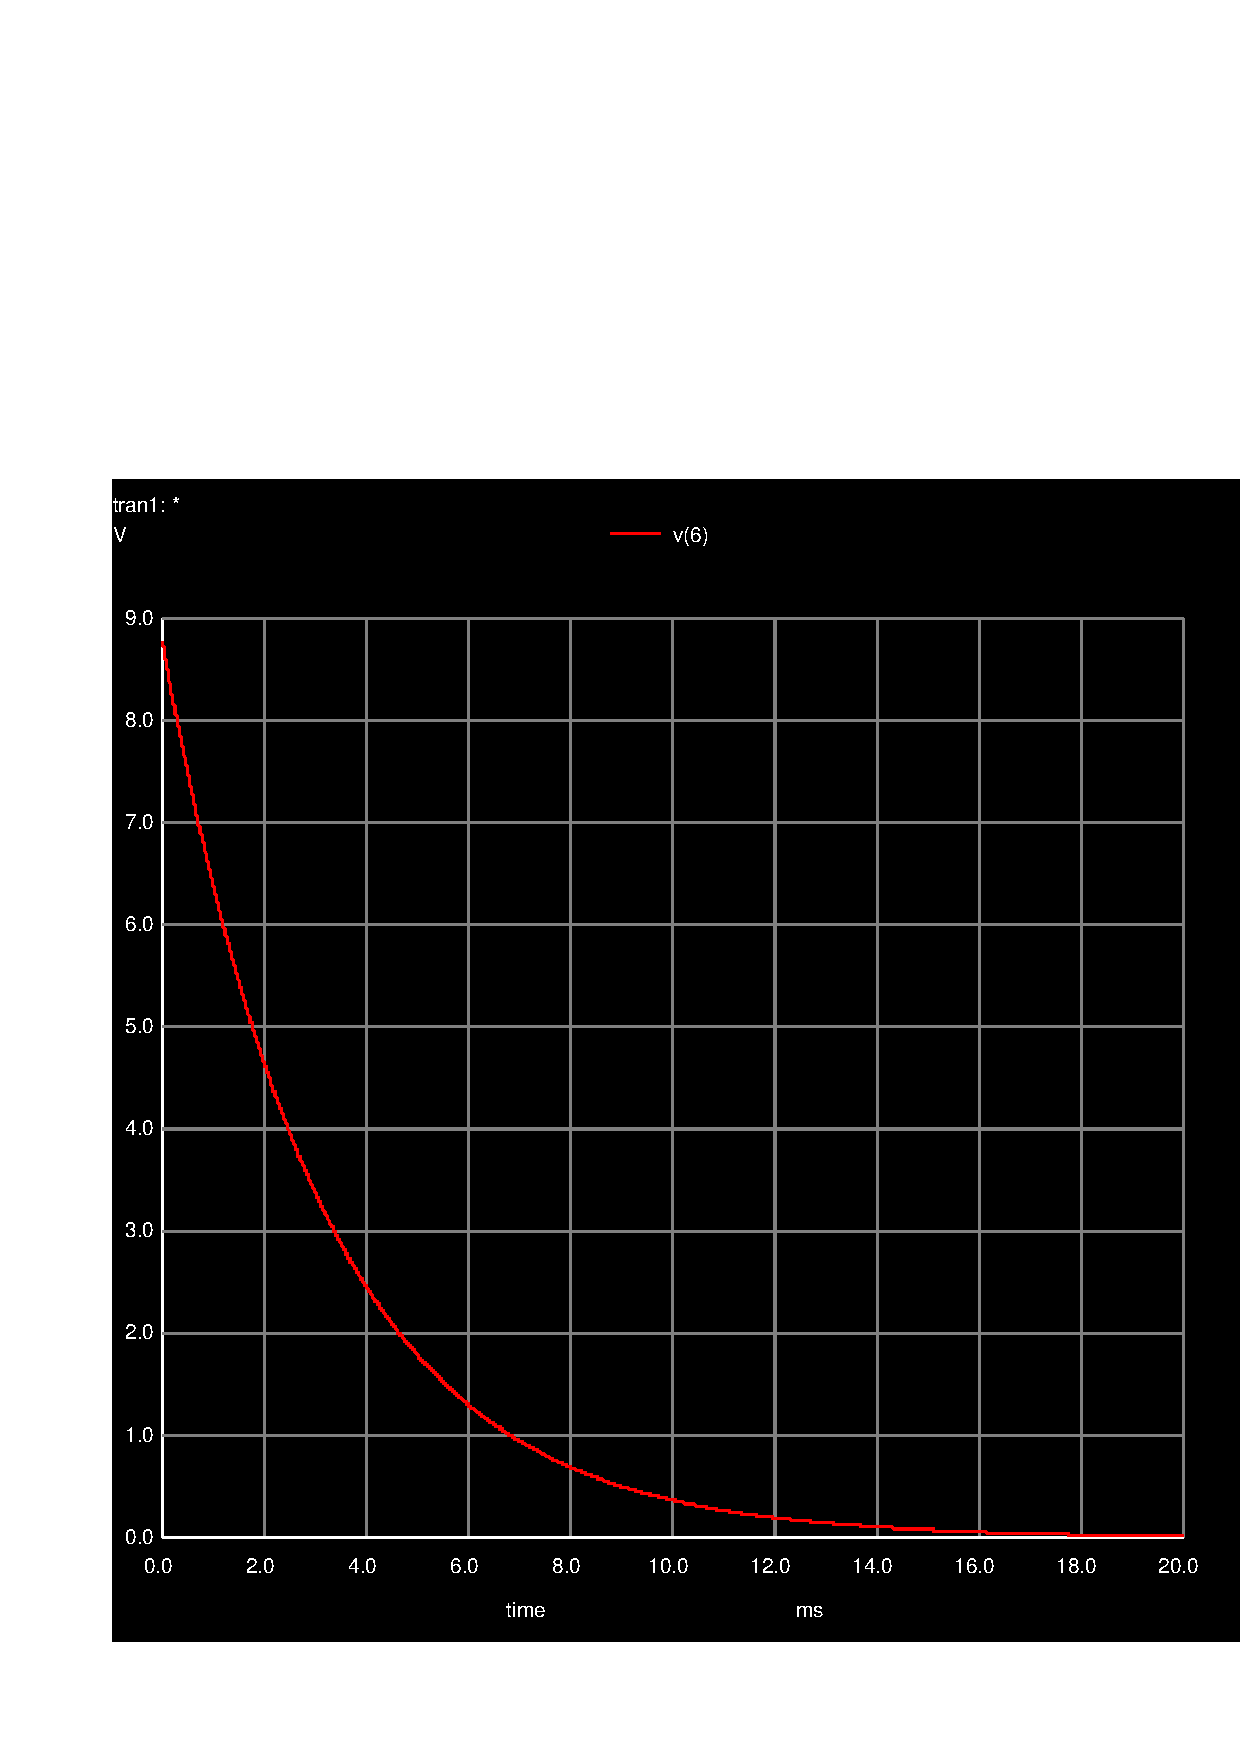
\includegraphics[width=0.4\linewidth]{trans.pdf}
  \caption{Natural solution for v(6)}
  \label{fig:sol_nat_spice}
\end{figure}

We started with the natural response of the circuit, that is, 
with $V_s=0$, to a boundary condition ($V_6$ and $V_8$ as determined 
in the previous section).
Using ngspice's transient analysis we were able to simulate the response. 
The value of $V_6$ is plotted in figure \ref{fig:sol_nat_spice}.
We can hence see total agreement between the theoretical results, 
from comparing the plots \ref{fig:naturalSolution} and 
\ref{fig:sol_nat_spice}.

\subsubsection{Total Response}

\begin{figure}[h] \centering
  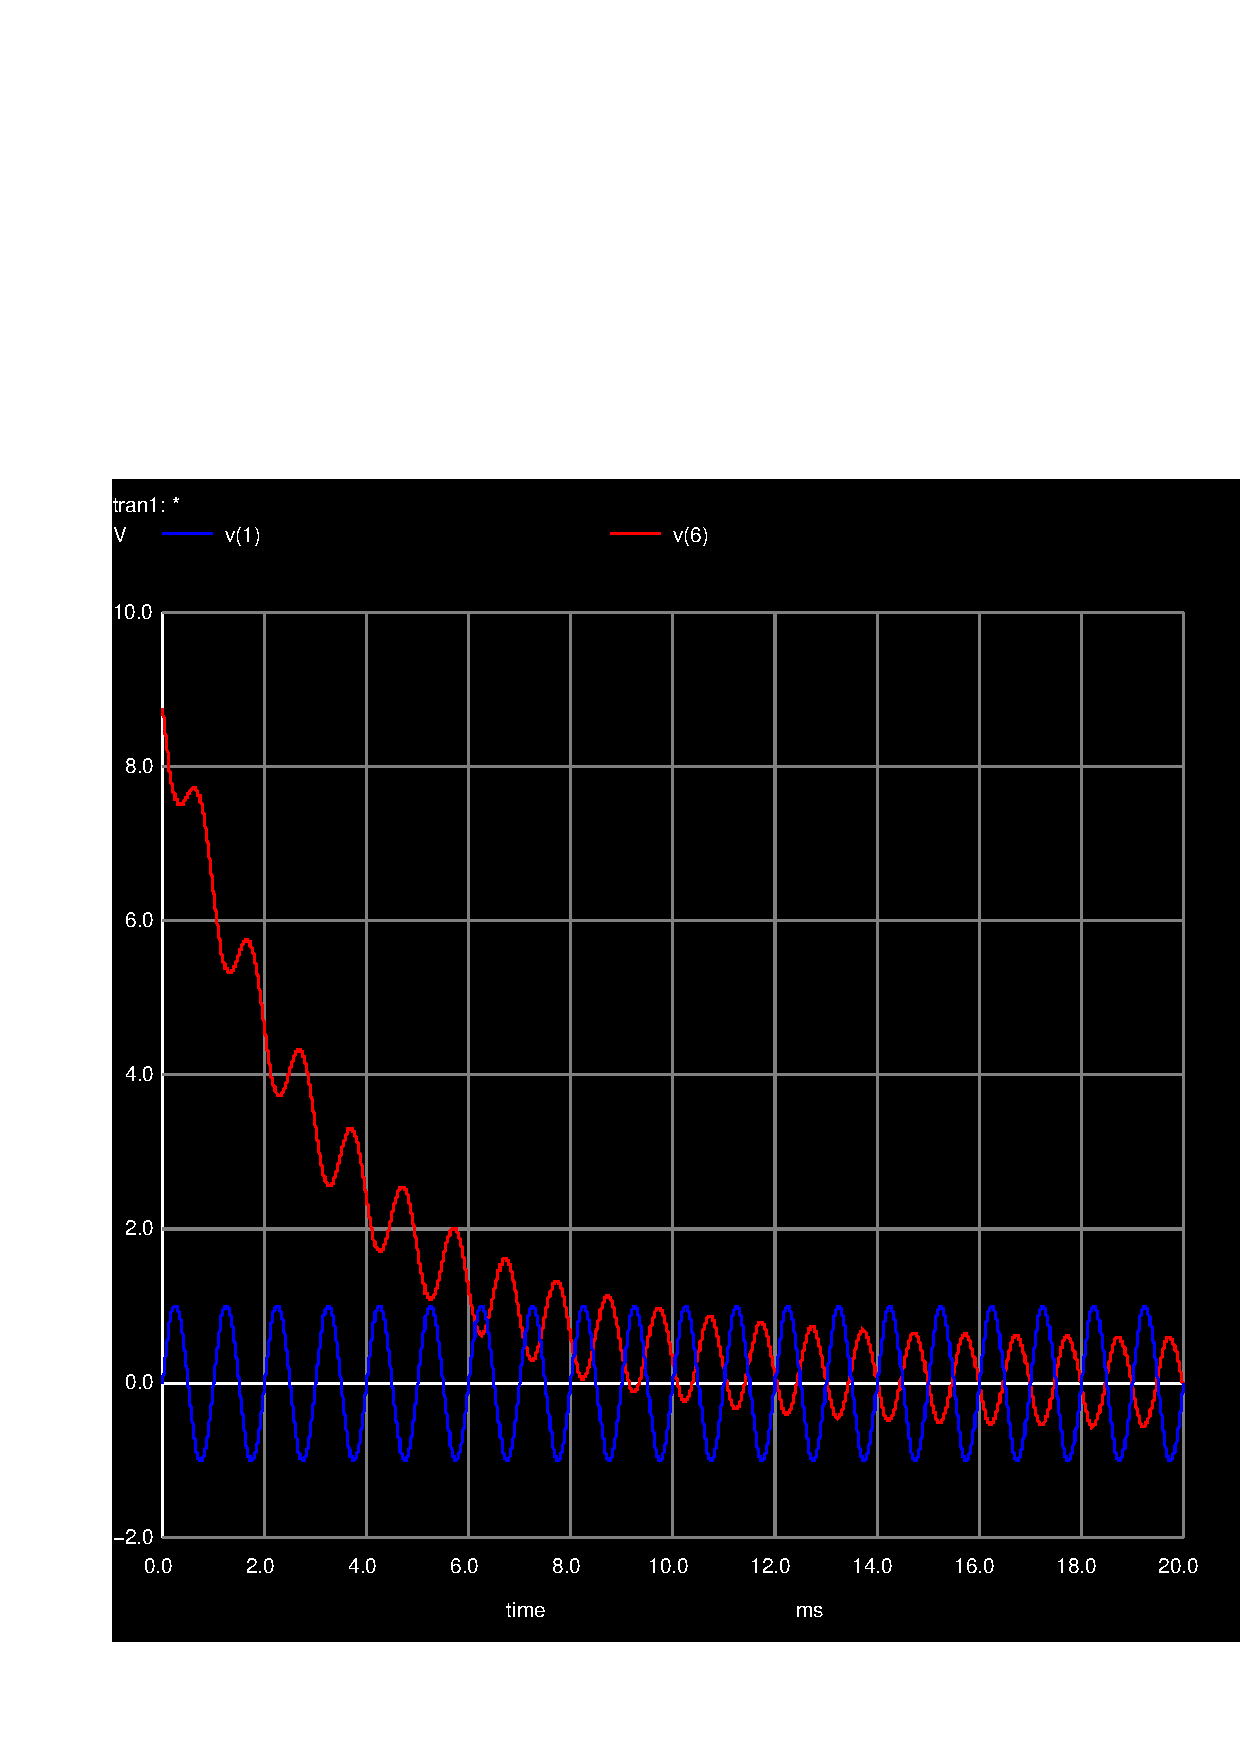
\includegraphics[width=0.4\linewidth]{solution.pdf}
  \caption{Total solution for v(6) and $V_s$}
  \label{fig:sol_tot_spice}
\end{figure}

Afterwards, we simulated the total response of the full circuit (natural 
+ forced) by assuming $V_s = sin(\omega t)$ (as explained in figure \ref{fig:circuit}), 
for a frequency of 1kHz.
The voltage in node 6 ($V_6$) and the input voltage ($V_s$) are plotted 
in figure \ref{fig:sol_tot_spice}. 
Once again the theoretical plot \ref{fig:sol_tot_spice} is 
indistinguishable from figure \ref{generalFinal}.


\subsubsection{Frequency Responce}

\begin{figure}[h] \centering
  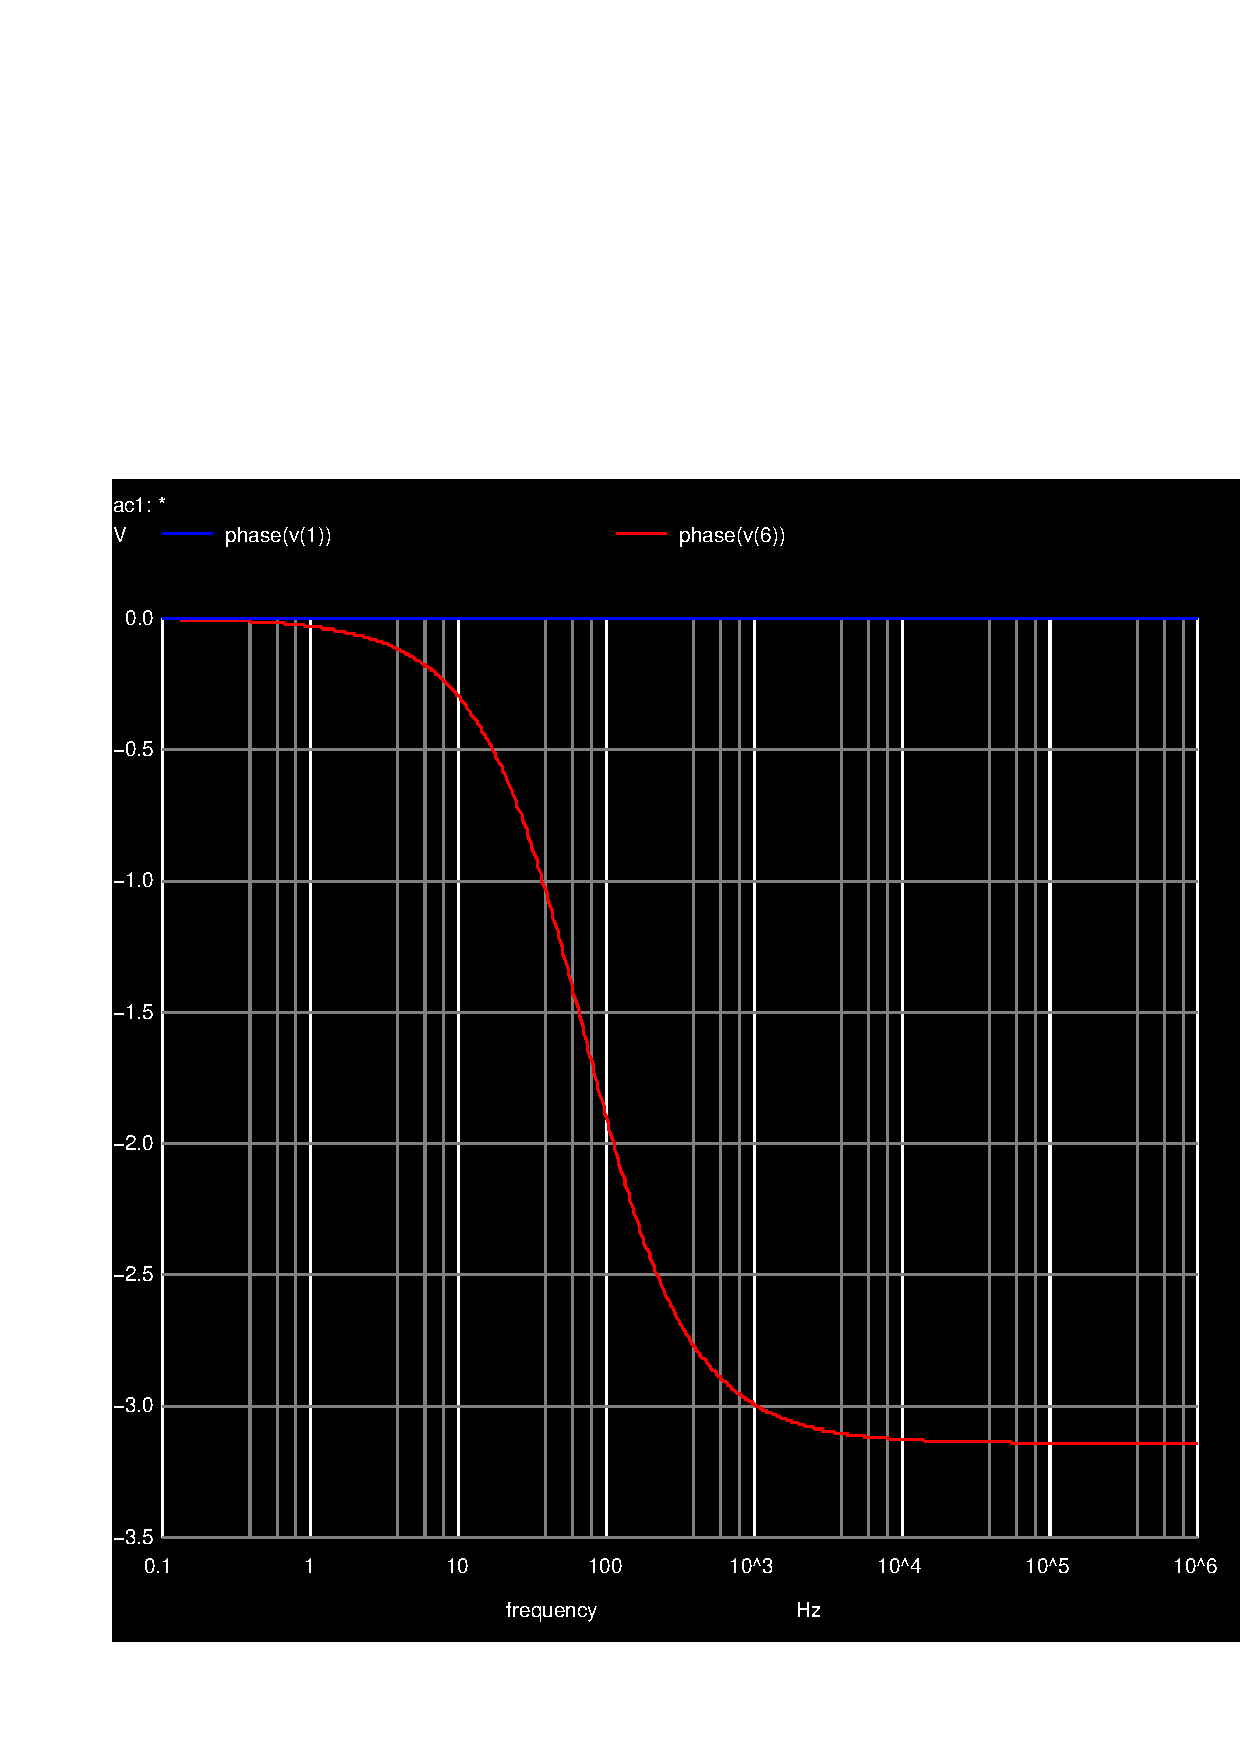
\includegraphics[width=0.4\linewidth]{acp.pdf}
  \caption{Total solution for v(6) and $V_s$ in degrees}
  \label{phase_spice}
\end{figure}

\begin{figure}[h] \centering
  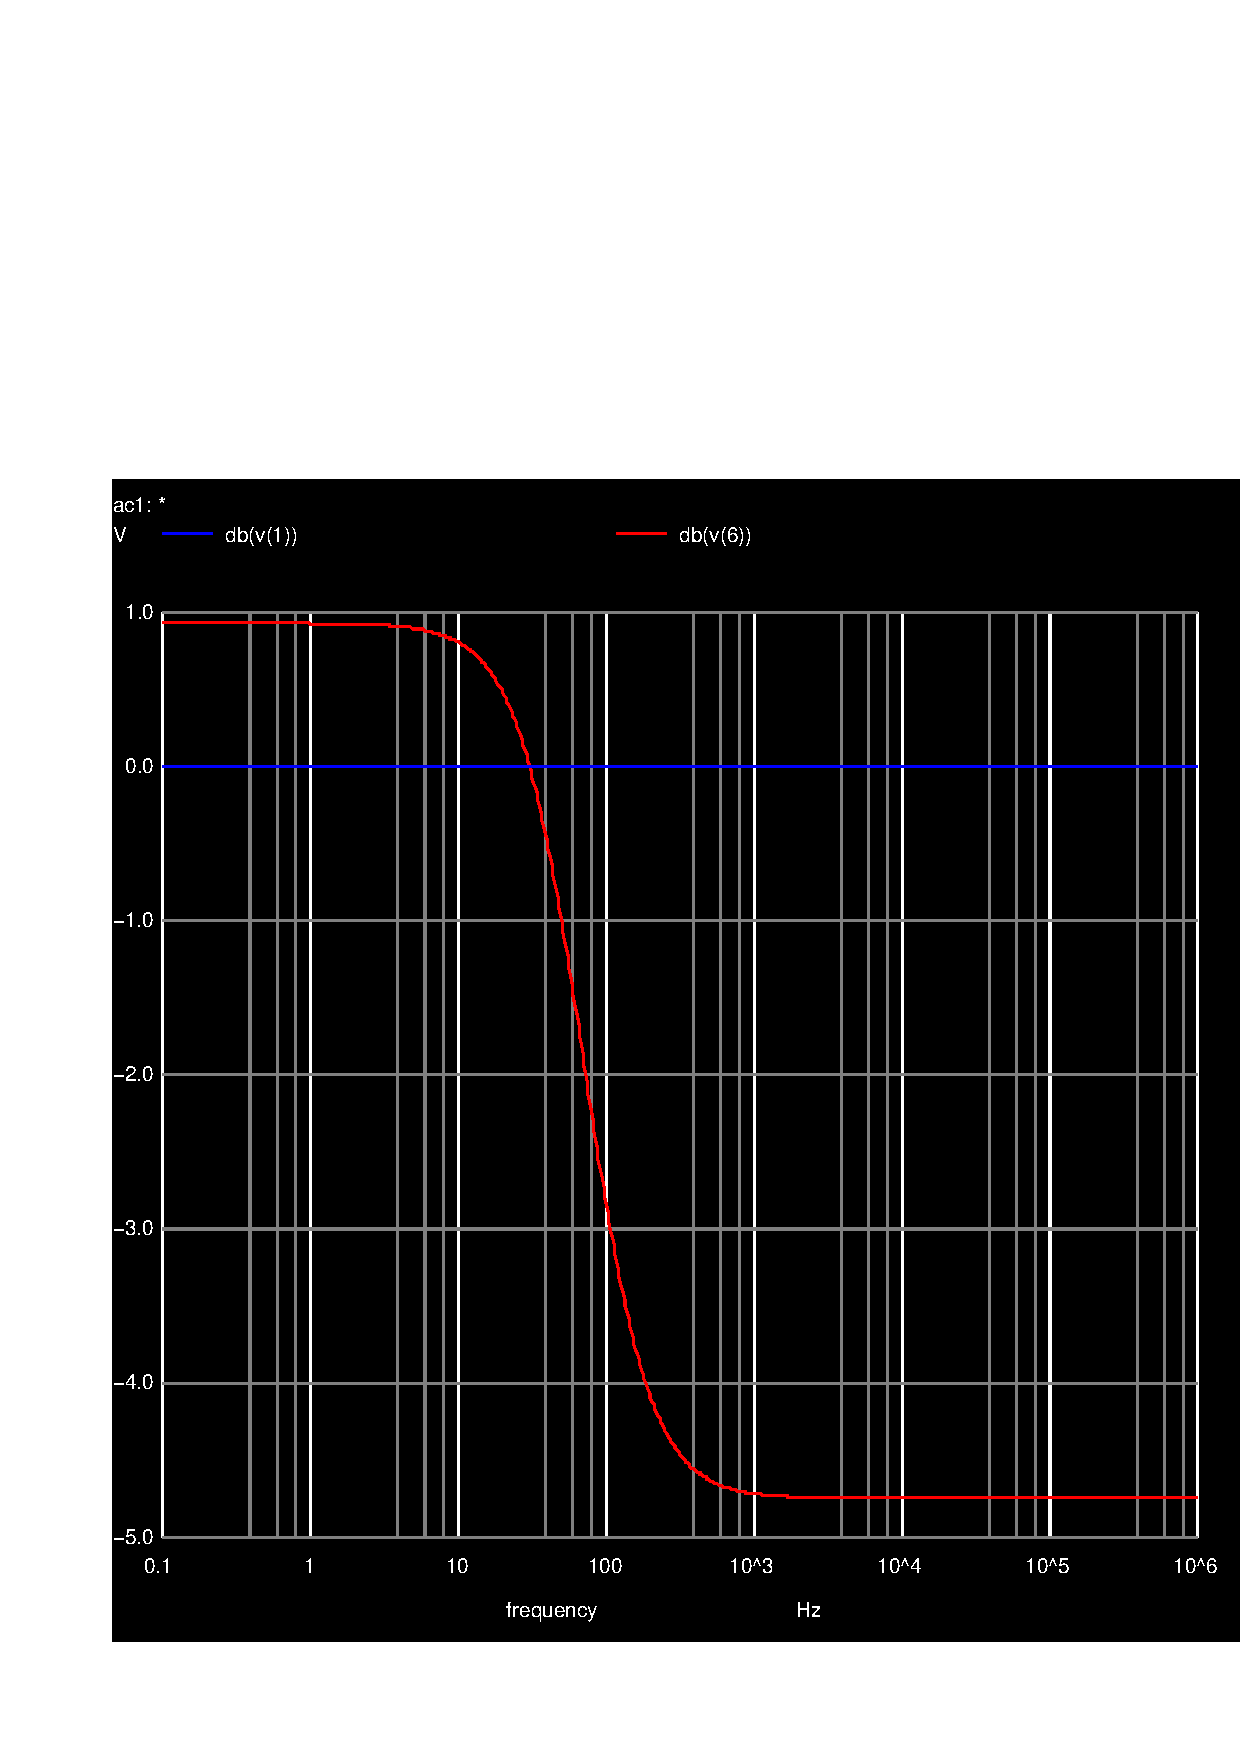
\includegraphics[width=0.4\linewidth]{acm.pdf}
  \caption{Amplitude response for v(6) and $V_s$ in dB}
  \label{amp_spice}
\end{figure}


Finally, with the goal of observing the low-pass filter nature 
of the capacitor, we simulated the circuit for various frequencies of 
$V_s$ (0.1Hz to 1MHz) and plotted the change in the phase (\ref{phase_spice}) 
and in the amplitude (\ref{amp_spice}) of $V_s$ and $V_6$. Note that the 
amplitude is expressed in dB's, justifying the negative values. Vs(f) is 0 as the ratio of it with itself is 1, therefore the logarithm is 0. As for V6(f), we can clearly observe the effect of the low-pass filter with the changes in output ratio for different frequencies.







%\lipsum[1-1]




